\section{Schlussteil}

\subsection{Ausblick}
Es konnte bereits während des Projektes ein gutes Ergebnis erzielt
werden. Dennoch wurden aufgrund der knappen Zeit nicht alle Ideen
umgesetzt. Weitere Möglichkeiten sehen wir im Bereich der nicht
verwendeten Daten und der Nutzung eines Offline-Learning-Verfahrens.
Des Weiteren besteht die Möglichkeit, die verwendeten Features auf ihre
Aussagekraft beziehungsweise Qualität zu untersuchen.

\subsubsection{Verwendung aller Daten}
Es werden bisher hauptsächlich Transaktionen berücksichtigt, die in Beziehung zu Gutscheinen stehen.
Bei diesen Transaktionen muss die Marke, die Kategorie oder das Unternehmen mit dem entsprechenden Gutschein übereinstimmen.
Diese Daten könnten in einem nächsten Iterationsschritt ebenfalls verwertet werden, wozu zunächst die folgenden Ansätze zusammengetragen wurden:
	
\begin{itemize}
\item Für jeden Kunden soll der komplette Umsatz pro Quartal bzw. pro Jahr ermittelt werden. Die Idee ist, dass der Umsatz das Kaufverhalten der Kunden beeinflusst.
 
\item Kunden, die in regelmäßigen Abständen einkaufen, kommen sehr wahrscheinlich wieder.
Beispielsweise werden wöchentlich die Nahrungsvorräte auf dem Heimweg von der Arbeit aufgefüllt.
Die Frequenz des Einkaufens kann über die Auswertung der Zeitangaben der Transaktionen ermittelt werden.

\item Clustering von oft zusammengekauften Marken, Kategorien und Unternehmen
ermöglicht weitere Features für die Kunden zu definieren.
Dies erfordert allerdings die Implementierung eines Clustering-Algorithmus
auf den Daten.
\end{itemize}

\subsubsection{Bewertung von Features}	
Sowohl bei den verwendeten Features als auch bei den oben vorgestellten Ideen ist bisher unklar, inwiefern diese Features das Kaufverhalten positiv, negativ oder überhaupt beeinflussen.
In unseren Vorträgen zur Veranstaltung ist zur Sprache gekommen, dass statistische Auswertungsverfahren zur Verfügung stehen, welche Aufschluss über die Qualität der Features treffen können. Da schlechte Features das Ergebnis negativ verfälschen können, ist dieser Ansatz besonders interessant.
Zur Umsetzung müsste die Korrelation zwischen den einzelnen Features und dem Wiederkaufverhalten gemessen werden. Auf dieser Basis kann ein Grenzwert festgelegt werden, ab dem ein Feature
zur Voraussage genutzt wird.

\subsubsection{Offline-Learning-Verfahren}	
Die Trainingsdaten, die von Kaggle für die Aufgabenstellung bereitgestellt werden, sind konstant und werden 
nicht um neue Trainingsdaten erweitert.
Daher ist es nicht zwingend notwendig, dass diese inkrementell gelernt werden.
Zurzeit nutzen wir allerdings ein Online-Learning-Verfahren zur Erstellung des Modells.
Wie im Abschnitt \ref{subsubSec:MachineLearning} beschrieben, hat dies zum Nachteil,
dass die Reihenfolge der Trainingsdaten Einfluss auf die Generierung des Modells hat. 
Daher wäre es wünschenswert ein Offline-Learning-Verfahren anstelle des von uns benutzten Online-Learning-Verfahrens zu nutzen.
Aufgrund der begrenzten Zeit, die uns zur Lösung des Problems zur Verfügung stand, haben wir keine Implementierung eines Offline-Learning-Verfahrens vollständig ausprobieren können.
Dies wäre somit ein Punkt, bei dem wir uns noch Verbesserungspotenzial erhoffen.

\subsection{Fazit}
Insgesamt verschafften uns die Veranstaltung und das Projekt einen guten Gesamtüberblick über das Themengebiet Big-Data.
Dabei mussten wir vor allem zu Beginn des Projekts viel Aufwand in das Grundverständnis investieren, da wir das Thema zuvor noch nicht behandelt hatten.
Die Seminarvorträge im Laufe des Semesters waren dabei sehr hilfreich und passten gut zu dem von uns gewählten iterativen Vorgehen.
Sofern im Rahmen eines Vortrags eine neue und für uns relevante Technologie vorgestellt wurde, haben wir diese in der nächsten Iteration berücksichtigt.  

Bei den Web-Services können wir in der Cloud von Amazon Jobs auf großen Datenmengen ausführen, was mit unseren normalen Maschinen nicht möglich gewesen wäre.
Diese Möglichkeit wird auch von vielen Unternehmen genutzt, sodass ein Einblick in die Praxis für uns sehr interessant war.
Durch unsere Nachlässigkeit wurde auch das von Amazon gesponsorte Kapital dezimiert,
nachdem der Cluster mehrere Tage nicht terminiert wurde.

Der allgemeine Eindruck von AWS ist gemischt. 
Nachteilig sind die langen Wartezeiten bis Probleme mithilfe von Log-Meldung
analysiert werden können. 
Bei Laufzeiten von mehreren Stunden stören kleine Verzögerungen nicht.
Allerdings sind die langen Wartezeiten beim Testen von kurzen Skripts
ziemlich hinderlich. 
Des Weiteren ist der Einstieg schwer, weil eine genaue Dokumentation der Amazon-Hive-Befehle nicht vorhanden ist.
Ebenso haben wir eine intuitive Benutzeroberfläche vermisst.
Uns gelang es dennoch, durch Recherchen alle nötige Skripte zu erstellen und abzuändern, um Tabellen zu generieren und die Anfragen fehlerfrei auszuführen.
Der große Vorteil von AWS liegt in der Möglichkeit, sehr große Datenmengen zu verarbeiten.
Außerdem kann die Performance der genutzten Systeme dem 
Anwendungsfall angepasst werden, was eine einfache Skalierungsmöglichkeit bietet.
Diese Vorteile konnten wir aufgrund der beschränkten Datenmenge in unserem
Projekt nicht ausnutzen

Insgesamt konnten wir durch den Einsatz verschiedener Technologien wie MapReduce oder Hive und Data-Mining-Verfahren ein deutlich besseres Ergebnis als die Gruppe im Vorjahr erreichen. Den Fortschritt über die Iterationen zeigt das folgende Diagramm.
\todo[inline]{Fabian, Lutz: Hier wäre ein kurzes Fazit der Data-Mining-Verfahren sinnvoll.}

Neben dem im Implementationskapitel vorgestellten Regression-Verfahren haben wir auch ein Klassifizierungs-Verfahren benutzt,
desen Implementierung wir nicht weiter vorgestellt haben. In den durchgeführten Tests erzielt das Klassifizierungs-Verfahren
aber in Kaggle eine geringere Punktzahl, daher können wir abschließend sagen, dass das gewählte Regressions-Verfahren in
Anbetracht der erzielten Punktzahl eine gute Wahl war.

Für die Implementierung der Data-Mining-Verfahren haben wir Vowpal Wabbit genutzt. Mit Vowpal Wabbit liesen sich die
gewählten Data-Mining-Verfahren - ohne großen Aufwand zur Einarbeitung - nutzen. Als Negativpunkt ist uns aufgefallen, dass
sich Vowpal Wabbit nicht einfach in Hadoop oder in AWS nutzen lässt. Daher können wir abschließend sagen, dass Vowpal Wabbit
zur Einarbeitung in das Thema Data-Mining sicher ein gutes Werkzeug ist, aber für das Arbeiten mit Big Data eigentlich nicht
geeignet ist.

Das nachfolgende Diagramm zeigt, wie sich unsere Platzierung innerhalb der einzelnen Iterationen verändert hat:

\begin{figure}[H]
\centering
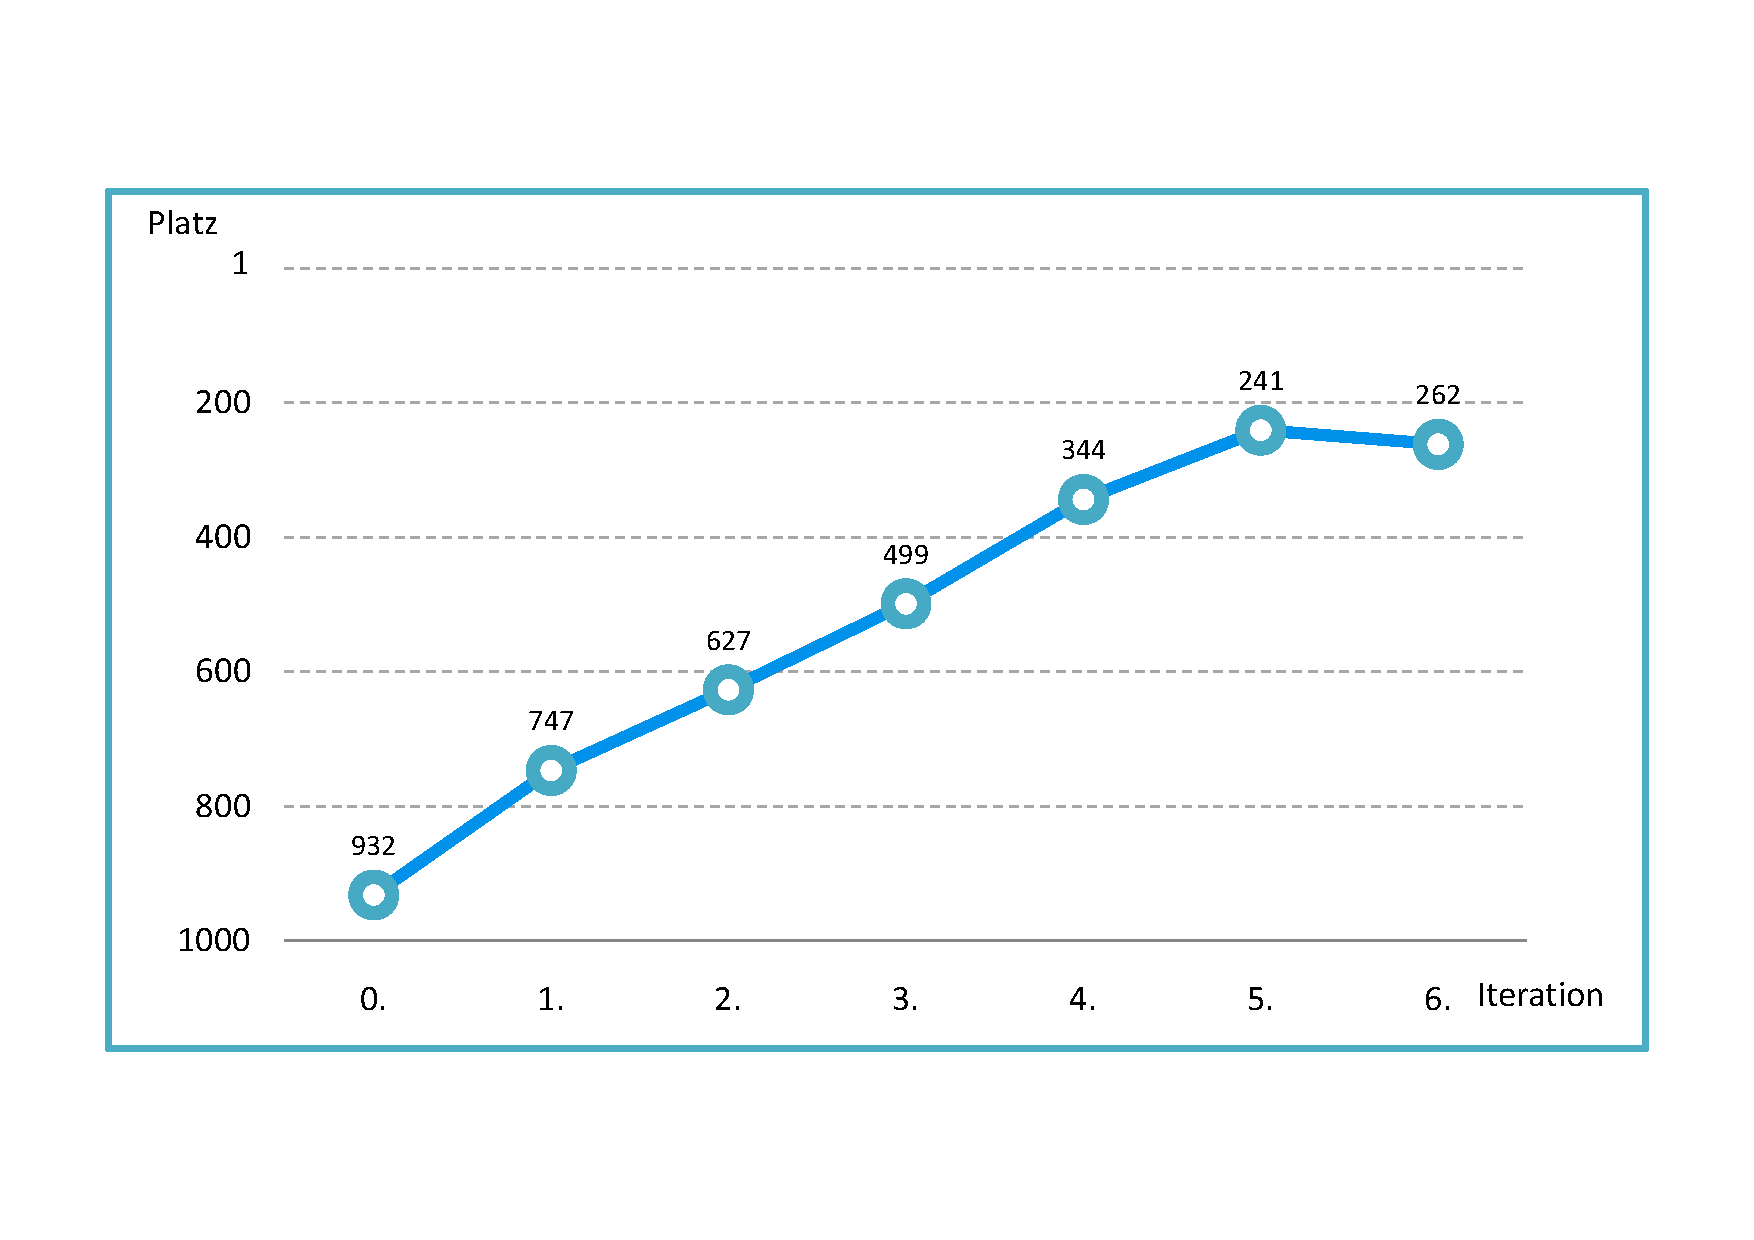
\includegraphics[width=0.85\linewidth]{Bilder/Trenddiagramm_Platzierungen}
\caption{Trenddiagramm unserer Kaggle-Platzierung}
\label{fig:Trenddiagramm_Platzierungen}
\end{figure}

Wie im Diagramm zu sehen, konnte mit jeder der 5 ersten Iterationen die Qualität der Vorhersage verbessert werden. In Iteration 4 konnten wir die Ergebnisse der Gruppe aus dem Vorjahr schlagen und haben letztendlich mit Iteration 5 unsere bisher beste Platzierung erreicht.

Die Auswahl eines Projektes auf der Plattform Kaggle.com, hatte für uns den besonderen Vorteil, dass wir unsere Ergebnisse direkt bewerten lassen konnten, auch wenn der Wettbewerb bereits beendet war. So konnte nach jeder Änderung geprüft werden, ob die Vorhersage verbessert wurde oder nicht. Zudem Bestand hier die Möglichkeit, sich mit Data-Mining Experten zu messen.

Generell gab die Veranstaltung einen guten Einstieg in die Verarbeitung großer Datenmengen und die dafür nötigen Werkzeuge. Es bleibt die Erkenntnis das es ein sehr umfassendes Gebiet ist, so dass für ein erfolgreiches Arbeiten in dem Bereich mehr als eine Veranstaltung nötig ist, um einen wirklichen Einstieg zu schaffen.
